\textbf{Цель работы: }\\
1) определить изменения температуры углекислого газа 
при протекании через малопроницаемую перегородку при разных начальных 
значениях давления и температуры;\\
2) вычислить по результатам опытов коэффициенты 𝑎 и 𝑏 модели Вандер-Ваальса.\\ \indent
\textbf{Оборудование: }трубка с пористой перегородкой; труба Дьюара; термостат
жидкостной; дифференциальная термопара; вольтметр универсальный (мультиметр);
балластный баллон; манометр.\\ 

\section*{Теоретические сведения}
\indent
\indent{Эффектом Джоуля–Томсона называется изменение температуры газа, медленно
просачивающегося из области высокого в область низкого давления в условиях 
тепловой изоляции. Коэффициентом Джоуля-Томсона называется величина:}
\begin{equation}
    \mu_{\text{д-т}} = \frac{\Delta T}{\Delta P} 
\end{equation} 
Выведем некоторые теоретические соотношения:
$$Q=0 \rightarrow \delta A = -\Delta U \rightarrow P_1 V_1-P_2 V_2 = 
(U_2 + \frac{\mu {\upsilon_2}^2}{2})-(U_1 + \frac{\mu {\upsilon_1}^2}{2})$$\\
Молярная энтальпия: $H = U+PV$, тогда 
$$H_1 - H_2 = \frac{\mu ({\upsilon_2}^2 - {\upsilon_1}^2)}{2}$$ 
Однако кинетическая энергия газа оказывается пренебрежимо малой, поэтому
$$H_1 \approx H_2$$
Рассмотрим реальный газ как газ Ван-дер-Ваальса:
$$\left ( P+\frac{a}{V^2}\right )(V-b) = RT$$
$$U = C_\text{v}T-\frac{a}{V}$$
Тогда энтальпия:
\begin{equation} \label{eq:entalp}
    H = U+PV=C_{\text{v}}T+RT\frac{V}{V-a} - \frac{2a}{V}
\end{equation}
При этом для упрощения вычислений будем считать газ разряженным и 
считать объем по формуле Клайперона-Менделеева $V \approx \frac{RT}{P}$, 
а также с учетом того, что $b \ll V$ из \ref{eq:entalp} получаем:
\begin{equation} \label{eq:entalpy}
H \approx C_{\text{P}}T + P \left (b- \frac{2a}{RT} \right )
\end{equation}
Так же будем считать изменения температуры в опыте небольшим 
$\frac{\Delta T}{T} \ll 1$. Тогда полагая $\Delta H = 0$ из \ref{eq:entalpy}:
\begin{equation}\label{eq:mu}
    \mu_{\text{д-т}} = \frac{\Delta T}{\Delta P} \approx -
    \frac{b - \frac{2a}{RT}}{C_{\text{P}}}
\end{equation}
Из \ref{eq:mu} видно, что существует такая температура (\emph{температура инверсии}),
при которой знак эффекта меняется:
\begin{equation}\label{eq:temperature}
    T_{\text{инв}} = \frac{2a}{Rb}
\end{equation}

\section*{Экспериментальная установка}
Схема установки для исследования эффектов Джоуля-Томсона в углекислом газе 
представлена на ниже.\\
\begin{figure}[h!]\label{fig:setup}
    \centering
    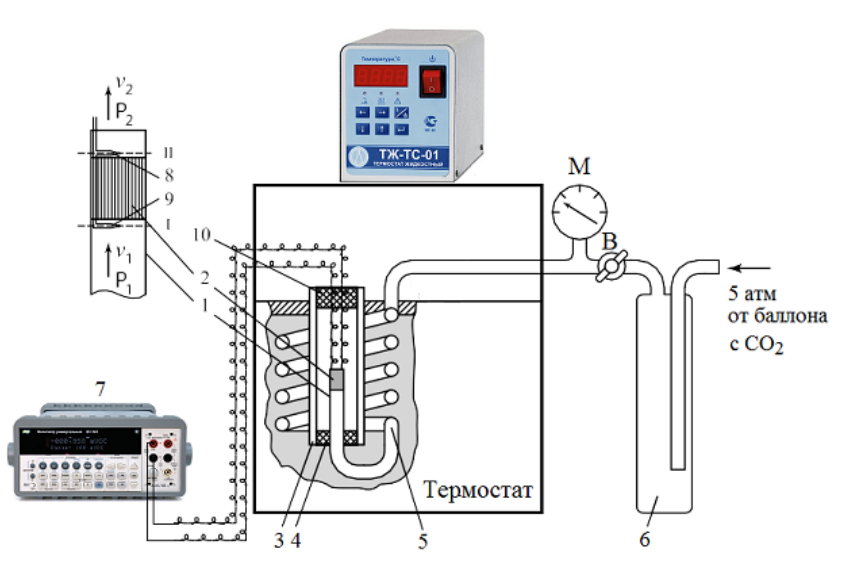
\includegraphics[width=15cm,height=10cm]{установка.png}
    \caption{Экспериментальная установка для исследования эффектов Джоуля-Томсона}
\end{figure}

\indent
Через турбку 1,сделанной из стали и потому обладающей малой теплопроводностью и
содержащей на конеце пористую перегородку 2, пропускается исследуемый 
газ - двуокись углерода $CO_2$. Углекислый газ под повышенным давлением
попадает в трубку через змеевик 5 из баллона 6. Змеевик в свое время 
медленно нагревает проходящий через него газ до температуры воды в термостате, 
который поддерживает ее постоянной с точностью $\pm 0.1^{\circ}C$. 
Манометр М измеряет разность давлений внутри трубки и снаружи. 
Разность температур газа до и после перегородки измеряется дифференциальной 
термопарой медь-констант, концы которой подключены к вольтметру. Если концы 
термопары имеют разную температуру, то в цепи возникает разность потенциалов, 
которая и измеряется вольтметром.



%западники(чаадаев) и славянофилы(аксаков хомяков тургенев)
%их противоборство(середина 19 века)

%цивизационная модель якова
